\documentclass[final,t]{beamer}
\mode<presentation>{ \usetheme{Major} }
\usepackage{times}
\usepackage{amsmath,amsthm, amssymb, latexsym}
\boldmath
\usepackage[english]{babel}
\usepackage{relsize}
\usepackage{multirow}
%\usepackage{qtree}
\usepackage{stmaryrd}
\usepackage{booktabs}

%  \usepackage[font=small,format=plain,labelfont=bf,up,textfont=it,up]{caption}
\usepackage[font=normalsize,labelfont=small,bf,margin=2cm]{caption}
\usepackage[latin1]{inputenc}
\usepackage[orientation=portrait,size=a0,scale=1.4,debug]{beamerposter}
\usepackage{color,listings}
\usepackage{calc,xcolor}
\usepackage[absolute,overlay]{textpos}
\usepackage{smartdiagram}
\usepackage{wrapfig}
\usepackage[many]{tcolorbox}
\usepackage{tikz}
\usetikzlibrary{shadings}


\long\def\omitit#1{} % used to comment-out /remove text at compile-time.

%\definecolor{lightblue}{rgb}{.85,.85,1} % 217 217 255
%\definecolor{lightorange}{rgb}{1,.8,.6} % 255 204 153
%\definecolor{lightgreen}{rgb}{.77,.91,.5} % 196 232 128
%\definecolor{lightyellow}{rgb}{1,.98,.6} % 255 250 153
%\definecolor{prussianblue}{rgb}{0.0,0.19,0.33}
%\definecolor{gold}{rgb}{0.6,0.4,0.08}


%\setbeamercolor{caption name}{fg=prussianblue} %''Figure'' titles colour
\setbeamercolor{caption name}{fg=britishRacingGreen} %''Figure'' titles colour

\makeatletter
\pgfdeclarehorizontalshading{beamer@headfade}{5.4375ex+490pt}
{%
  color(0cm)=(lightblue);
  % color(15cm)=(lightblue);
  color(45cm)=(lightyellow);
  color(\paperwidth)=(gold)%
}
\addtoheadtemplate{\pgfuseshading{beamer@headfade}\vskip\dimexpr 0pt-52ex}{}
\makeatother


\newsavebox\CBox
\newenvironment{ColorBox}[3][black]{
    \par\noindent
    \def\borderColor{#1}\def\bgColor{#2}
    \begin{lrbox}{\CBox}
    \minipage{#3-2\fboxsep-2\fboxrule}
}{
    \endminipage\end{lrbox}%
    \fcolorbox{\borderColor}{\bgColor}{\usebox\CBox}\par
}

\lstset{language=java}
\lstset{breaklines=true}
\lstset{showstringspaces=false}
\lstset{tabsize=3}
\lstset{basicstyle=\ttfamily\scriptsize}
\lstset{breakautoindent=true}
\lstset{postbreak=\space}
%\lstset{commentstyle=\color{XcodeComments}}
%\lstset{keywordstyle=\color{XcodeKeywords}}
%\lstset{stringstyle=\color{XcodeStringstyle}}

%%%%%%%%%%%%%%%%%%%%%%%%%%%%%%%%%%%%%%%%%%%%%%%%%%%%%%%%%%%%%%%%%%%%%%%%%%%%%%%%%5
\title[]{Text mining in Python for Evaluating the Ethical Foundations in Computer Science}
\author[Bonham-Carter]{Enpu You, Oliver Bonham-Carter, Janyl Jumadinova}
\institute{Depts of Computer Science, Allegheny College \\ Meadville, PA}
\webpage{https://csethics.allegheny.edu}
\mail{\{youe2, obonhamcarter, jjumadinova\}@allegheny.edu}


%%%%%%%%%%%%%%%%%%%%%%%%%%%%%%%%%%%%%%%%%%%%%%%%%%%%%%%%%%%%%%%%%%%%%%%%%%%%%%%%%
\begin{document}
    \begin{frame}{}
        \vspace*{2mm}
        \begin{columns}[t]
        	\begin{column}{1\linewidth}
%%%%%%%%%%%%%%%%%%%%%%%%%%%%%%%%%%%%%%%%%%%%%%%%%%%%%%%%%%%%%%%%%%%%%
%
% Center column - Context
%
%%%%%%%%%%%%%%%%%%%%%%%%%%%%%%%%%%%%%%%%%%%%%%%%%%%%%%%%%%%%%%%%%%%%%

%%%%%%%%%%%%%%%%%%%%%%%%%%%%%%%%%%%
%
% Project Objectives
%
%%%%%%%%%%%%%%%%%%%%%%%%%%%%%%%%%%%
                \begin{block}{\textsc{\textbf{Project Objectives}}}
				\vspace*{3mm}

				\omitit{
		\begin{wrapfigure}{r}{0.35\textwidth}
					\begin{figure}
						\centering
						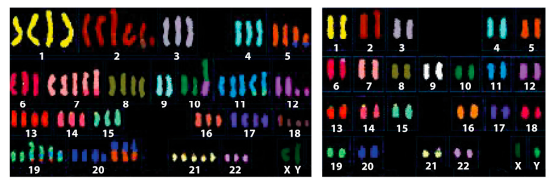
\includegraphics[scale = 1.4]{graphics/chromosomes.png}
                        \caption{\ref{fig:chromosomes}. \small A karyotype of cancer cells of relatively stable genome (Alberts, \emph{et al.}, Molecular Biology of the cell), right.}
                        \label{fig:chromosomes}
					\end{figure}
                        \end{wrapfigure} 
		}
                        We present an automated text-mining tool written in Python to measure the technical responsibility of students in computer science courses.

				\begin{itemize}
					\item Our tool automatically collects reflection documents written by students from their GitHub repositories.
					\item Then, using natural language processing analyzes them for ethical considerations based on pre-determined questions and criteria. 
					\item Using our tool, it is possible to see the progression of a single student's ethical thinking throughout a specific course and throughout the entire computer science curriculum, as well as, to have a grand view of all students' progress in developing an understanding of social responsibility in computer science across all levels of our courses. 

				\end{itemize}

                    \vspace*{6mm}
                \end{block}
			\end{column}
		\end{columns}

%%%%%%%%%%%%%%%%%%%%%%%%%%%%%%%%%%%%%%%%%%%%%%%%%%%%%%%%%%%%%%%%%%%%%

		\begin{columns}

%%%%%%%%%%%%%%%%%%%%%%%%%%%%%%%%%%%%%%%%%%%%%%%%%%%%%%%%%%%%%%%%%%%%%
%
% Left column - Context
%
%%%%%%%%%%%%%%%%%%%%%%%%%%%%%%%%%%%%%%%%%%%%%%%%%%%%%%%%%%%%%%%%%%%%%
            \begin{column}{.5\linewidth}
%%%%%%%%%%%%%%%%%%%%%%%%%%%%%%%%%%%
%
% Method
%
%%%%%%%%%%%%%%%%%%%%%%%%%%%%%%%%%%%
			\begin{block}{\textsc{\textbf{Teaching responsible computing}}}
				\vspace*{3mm}
%                  \begin{wrapfigure}{r}{0.5\textwidth}
				\omitit{
				\begin{figure}
					\centering
					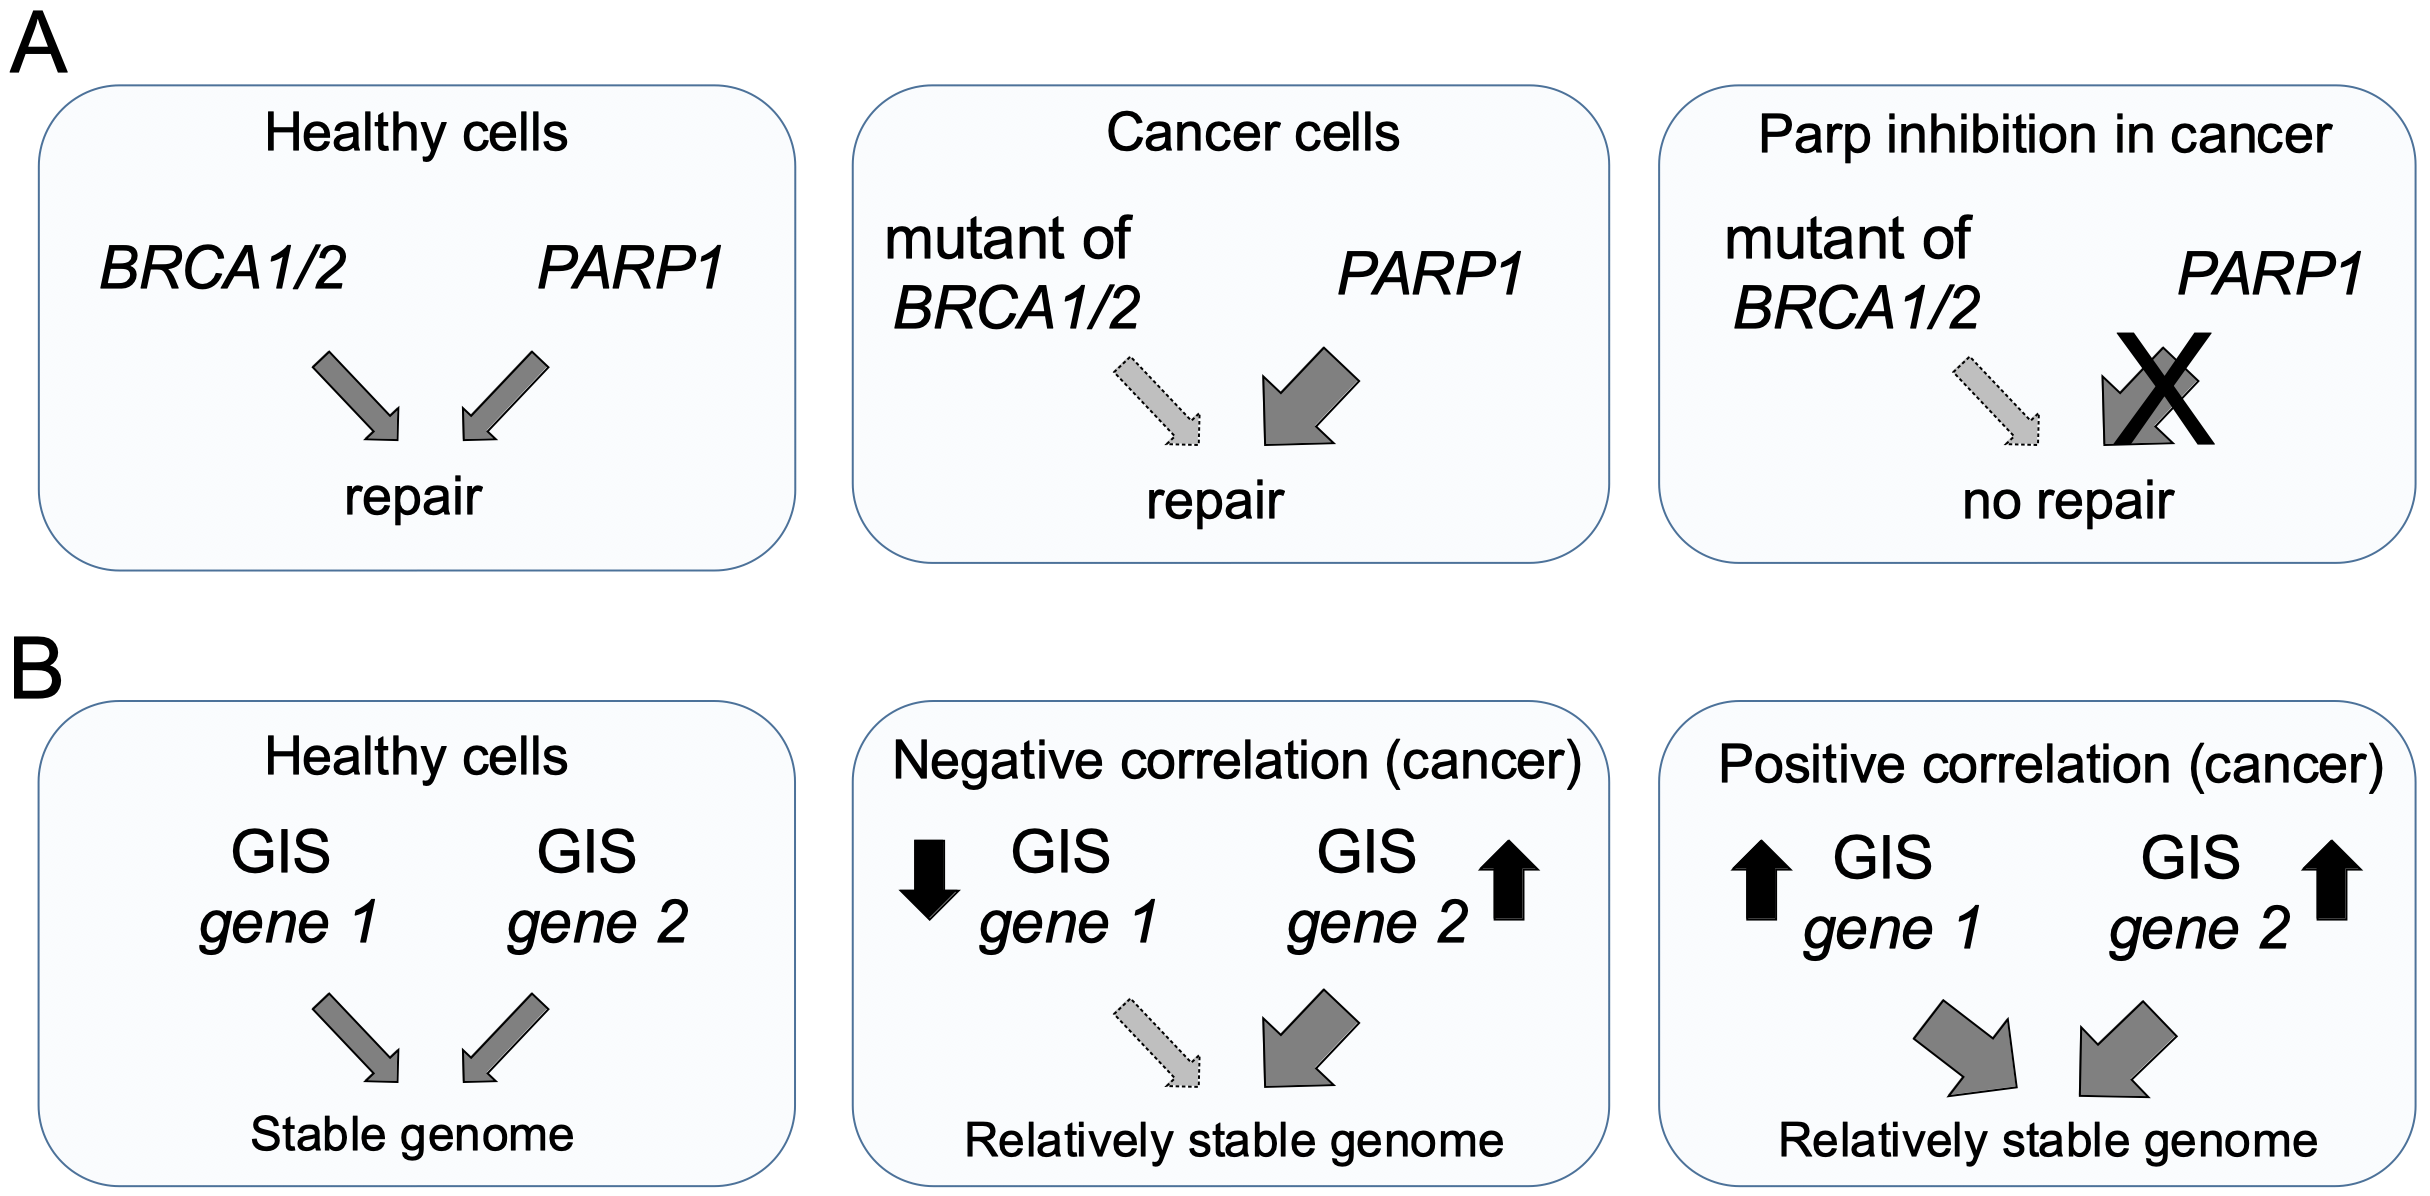
\includegraphics[scale = 0.6]{graphics/braca.png}
					\caption{\ref{fig:braca}. Co-Dependance by genes}
					\label{fig:braca}
%                  \end{wrapfigure}
					\end{figure}
				}
Teaching responsible computing is critical in developing software that produces a positive impact on our society, economy, and individuals.
				\begin{itemize}
					\item  Each application course in computer science at Allegheny integrates ethical considerations in its pedagogy.
					\item Broad learning categories include topics of internet health, ethics and responsible computing that are specific to each application course. 
					\item The delivery of these concepts include readings and class discussions, class and lab assignments with heavy software development emphasis. 
					\item Students  write reflection reports for these assignments that demonstrate their understanding of relevant issues,  ability to analyze and evaluate information, and their capacity for integrating the understanding and analysis of ethical thinking into their own work.
				\end{itemize}
				\vspace*{3mm}
			\end{block}
%%%%%%%%%%%%%%%%%%%%%%%%%%%%%%%%%%%
%
% Design
%
%%%%%%%%%%%%%%%%%%%%%%%%%%%%%%%%%%%

  %%%%%


			\begin{block}{\textsc{\textbf{Text Mining Tool to Determine Ethical Pedagogy}}}
			\begin{center}

 Random selection of ten data sets of breast cancer gene expression. 
				\begin{figure}
					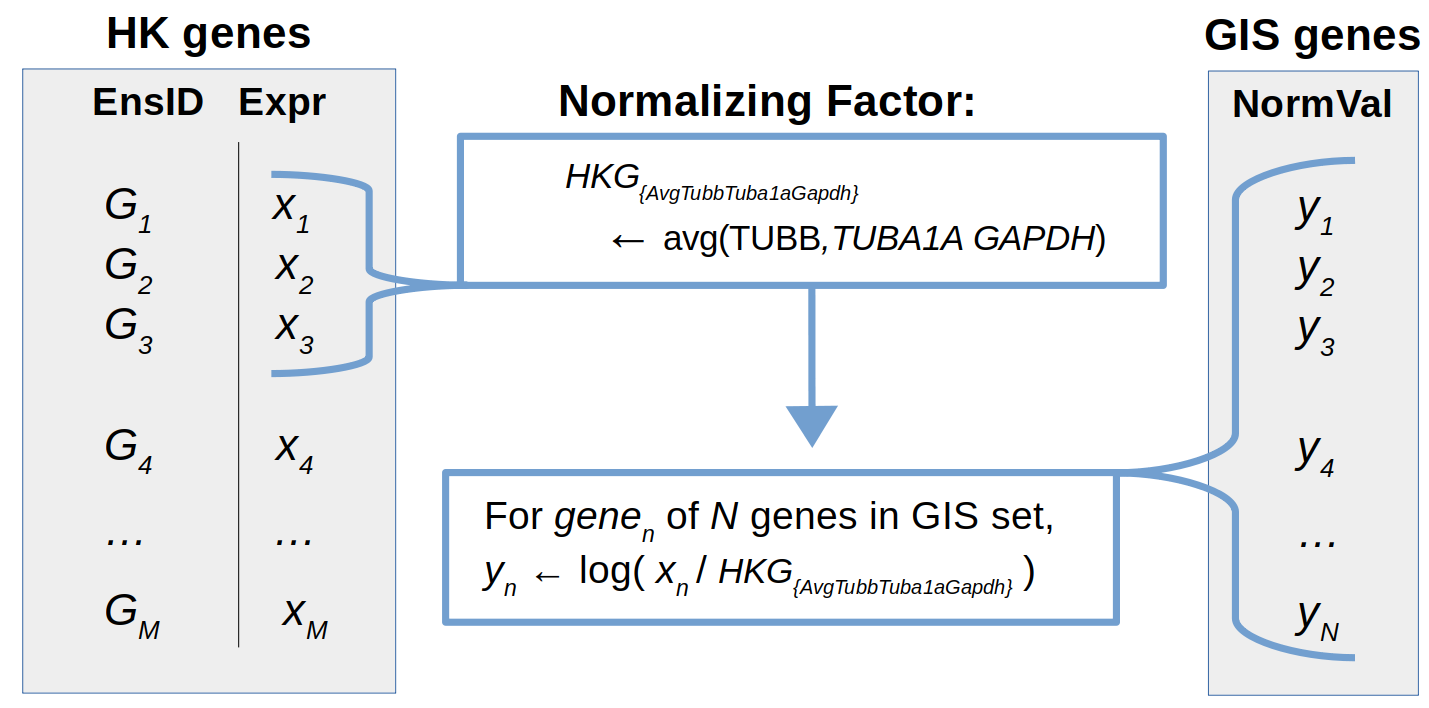
\includegraphics[scale = 0.60]{graphics/normFactor.png}
					\caption{\ref{fig:normFactor}. Determining the normalizing factors}
					\label{fig:normFactor}
				\end{figure}
				
				\begin{center}\end{center} % separation space between both figures
				
				\begin{figure}
					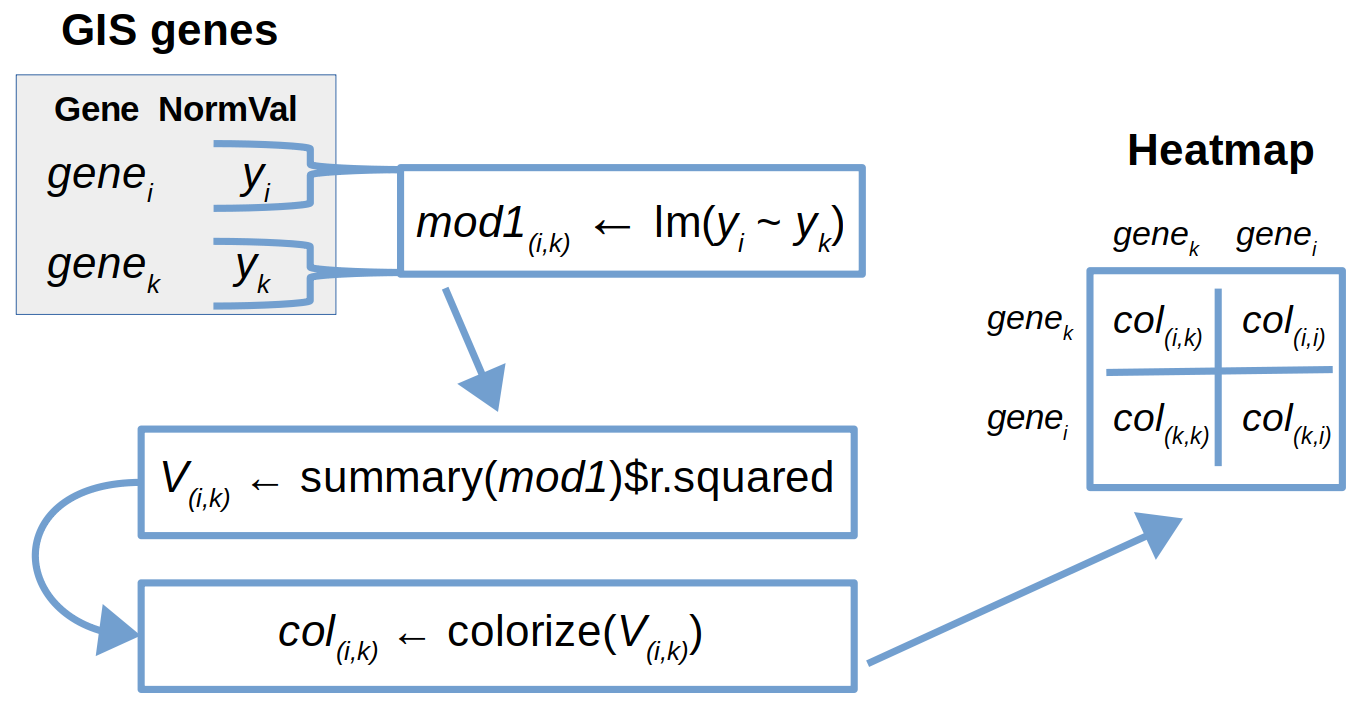
\includegraphics[scale = 0.60]{graphics/lm.png}
					\caption{\ref{fig:lm}. HouseKeeping genes to normalize data sets}
					\label{fig:lm}
				\end{figure}
			\end{center}

				\begin{itemize}
					\item  bla bla bla
					\item  bla bla bla
					\item  bla bla bla
				\end{itemize}
			\vspace*{3mm}
                \end{block}
	\end{column}

%%%%%%%%%%%%%%%%%%%%%%%%%%%%%%%%%%%%%%%%%%%%%%%%%%%%%%%%%%%%%%%%%%%%%
%
% Right column - Outcomes
%
%%%%%%%%%%%%%%%%%%%%%%%%%%%%%%%%%%%%%%%%%%%%%%%%%%%%%%%%%%%%%%%%%%%%%
	\begin{column}{.5\linewidth}
%%%%%%%%%%%%%%%%%%%%%%%%%%%%%%%%%%%
%
%
%
%%%%%%%%%%%%%%%%%%%%%%%%%%%%%%%%%%%

%			\begin{block}{\textsc{\textbf{Determining Normalization Factors}}}
%
%
%			\begin{center}
%				\begin{figure}
%					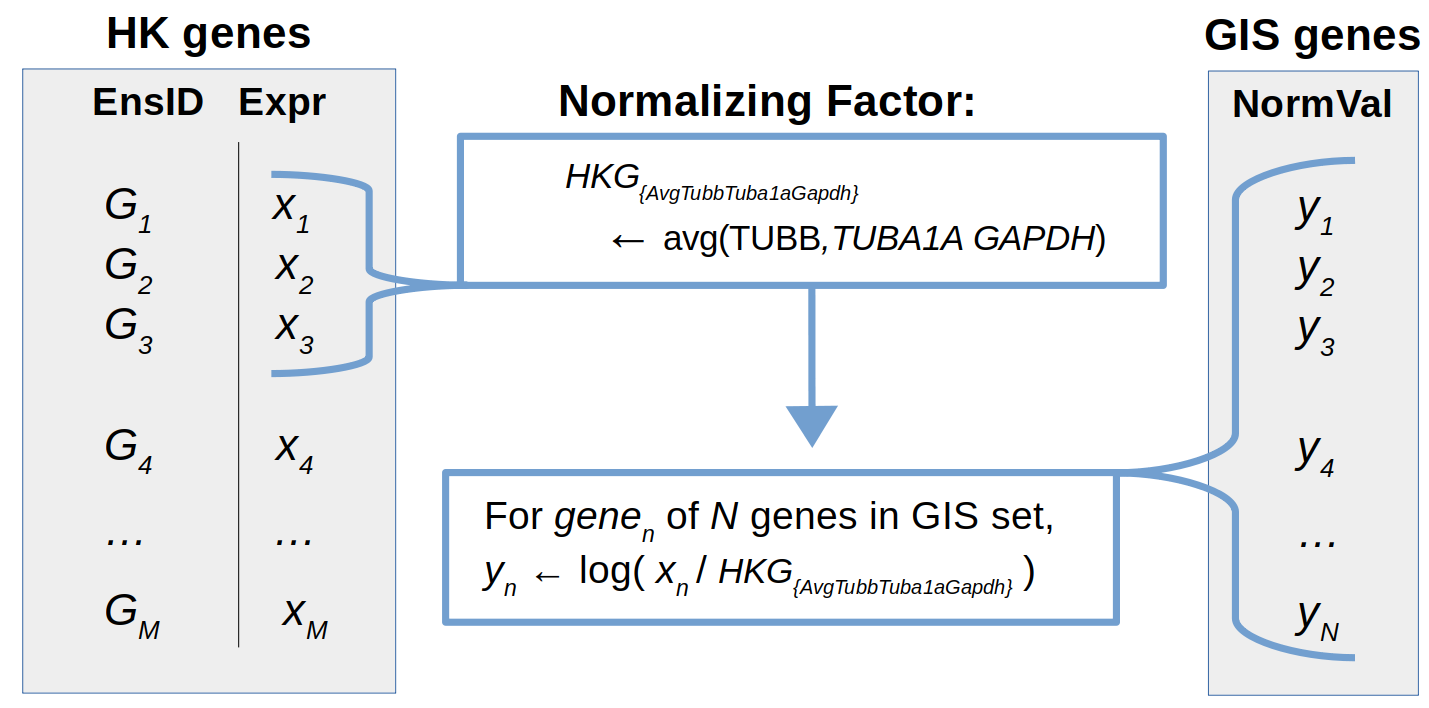
\includegraphics[scale = 0.6]{graphics/normFactor.png}
%					\caption{\ref{fig:normFactor}. Determining the normalizing factors}
%					\label{fig:normFactor}
%				\end{figure}
%			\end{center}
%			\begin{itemize}
%					\item bla bla
%					\item bla bla
%			\end{itemize}
%			\end{block}

		\begin{block}{\textsc{\textbf{Features}}}
			\vspace*{3mm}
			\begin{figure}
				\begin{tabular}{cc}
					\hspace*{5mm}

					\includegraphics[scale = 0.28]{graphics/R_geneExpression_A.png}
					\textbf{A.}
					&                     
					\includegraphics[scale = 0.28]{graphics/R_geneExpression_B.png}
					\textbf{B.}\\

					\includegraphics[scale = 0.28]{graphics/R_geneExpression_avgABC.png}
					\textbf{C.}
					&                      
					\includegraphics[scale = 0.32]{graphics/R_geneExpression_AVGG1.png}
					\textbf{D.}\\

					\includegraphics[scale = 0.28]{graphics/R_geneExpression_AVGG2.png}
					\textbf{E.}
					&                      
					\includegraphics[scale = 0.28]{graphics/R_geneExpression_AVGG3.png}
					\textbf{F.}\\
				\end{tabular}				
				\caption{\ref{tab:ge}. Heatmaps of R$^{2}$ values, derived from normalizing factors}
				\label{tab:ge}
			\end{figure}
			\begin{itemize}
				\item  bla bla bla
				\item  bla bla bla
				\item  bla bla bla
			\end{itemize}
			\vspace*{3mm}
		\end{block}
                %%%%%%%%%%%%%%%%%%%%%%%%%%%%%%%%%%%
                %
                % Sensors
                %
                %%%%%%%%%%%%%%%%%%%%%%%%%%%%%%%%%%%
		\begin{block}{\textsc{\textbf{Results}}}
			\vspace*{3mm}
			
%			\begin{wrapfigure}{l}{0.47\textwidth}
%				\centering
%				\includegraphics[width=0.35\textwidth]{assets/sensors.jpg}
%				\caption{Arduino board and sensors}
%			\end{wrapfigure}
			
			\begin{itemize}
				\item  bla bla bla
				\item  bla bla bla
				\item  bla bla bla				
			\end{itemize}
			\vspace*{3mm}
	\end{block}

%%%%%%%%%%%%%%%%%%%%%%%%%%%%%%%%%%%
%
% Results
%
%%%%%%%%%%%%%%%%%%%%%%%%%%%%%%%%%%%
	\begin{block}{\textsc{\textbf{Conclusions}}}
		\vspace*{3mm}

		\begin{itemize}
			\item  bla bla bla
			\item  bla bla bla
			\item  bla bla bla
		\end{itemize}
%		\begin{figure}
%			\includegraphics[scale = 2.5]{}
%			\caption{}
%			\end{figure}
		\vspace*{3mm}
	\end{block}
	\end{column}


	\end{columns}
	\end{frame}
\end{document}









%%%%%%%%%%%%%%%%%%%%%%%%%%%%%%%%%%%%
% Junk bin
% Do not delete the following code, but remove it from the project
%%%%%%%%%%%%%%%%%%%%%%%%%%%%%%%%%%%%



